% Aidan Hunt
% ME 498 K
% Spring 2023
% Homework 1

\documentclass{homework}
\usepackage[utf8]{inputenc}
\usepackage{amsmath}
\usepackage{amssymb}
\usepackage{braket}
\usepackage{bm}
\usepackage{caption}

% Packages for presenting code
\usepackage{listings}
\usepackage{pythonhighlight}


\lstdefinestyle{BashOutputStyle}{
  basicstyle=\footnotesize\ttfamily,
  numbers=none,
  frame=tblr,
  columns=fullflexible,
  backgroundcolor=\color{blue!10},
  linewidth=0.9\linewidth,
  xleftmargin=0.1\linewidth
}

% Packages for presenting output
\usepackage{hyperref}
\hypersetup{
    colorlinks=true,
    linkcolor=blue,
    filecolor=magenta,      
    urlcolor=blue,
    }

%use \question*{Title} to title a question

% make short commands for subproblem listing
\newcommand{\substart}{\begin{enumerate}[label={(\alph*)}]}
\newcommand{\subend}{\end{enumerate}}

%Instructor info
\newcommand{\hwname}{Aidan Hunt}
\newcommand{\hwemail}{ahunt94@uw.edu}

%Assignment type
\newcommand{\hwtype}{Homework}

%Class info
\newcommand{\hwclass}{ME 498 K}
\newcommand{\hwterm}{Spring 2023}

%Assignment specifics
\newcommand{\hwnum}{4}
\newcommand{\hwduedate}{April 28, 2023}

% \newcommand{\uu}	    {{\mathrm{\textbf{u}}}}

\begin{document}
\maketitle

In this homework, you will practice creating, manpipulating, and plotting NumPy arrays. Post questions about this assignment to the class discussion board for the fastest response. Submit your responses to problems 1) and 2) as separate files.

\question*{Airfoil Artist}

The general equation for the coordinates of a \href{https://en.wikipedia.org/wiki/NACA_airfoil}{symmetric NACA airfoil} with zero pitch and leading edge located at $(x,y) = (0,0)$ is given by:

\begin{equation}
    y = \pm 5ct [0.2969\sqrt{x/c} - 0.1260(x/c) - 0.3516(x/c)^2 + 0.2843(x/c)^3 - 0.1036(x/c)^4]
\end{equation}

where $c$ is the chord length (i.e., the distance from the leading edge to the trailing edge), $x$ is the position along the foil chord line (0 at leading edge, $c$ at trailing edge), and $y$ is the half-thickness of the foil at a given $x$ position. $t$ is the maximum thickness normalized by the chord length, and is specified by the digits in the symmetric airfoil name. For example, for a NACA 0018 airfoil, $t = 0.18$ because the maximum thickness of the airfoil is 18\% of the chord length.

In this problem, you will write a Python script that computes and plots the coordinates of an arbitary number of NACA airfoils, each with a specified chord and pitch angle. You will use NumPy arrays, and should consider NumPy functions that will help you build and manipulate these arrays.

\subsubsection*{Output Requirements}

You should define a function, \texttt{computeAirfoils()}, which takes name(s) of NACA airfoil profiles, the corresponding chord length(s), and the corresponding pitch angle(s) (in degrees), and produces the following output:
\begin{enumerate}
    \item \textbf{Returns} a \textit{single} 3-D NumPy array of floats that contains the \textit{full} profile coordinates of all airfoils. Each "page" of the array should represent a single airfoil. For each airfoil's "page", the first row should represent the $x$ coordinates of that airfoil, and the second row should represent the $y$ coordinates of the airfoil. The quarter-chord position of each airfoil should be located at $(x,y) = (0,0)$.
    \item Produce a single plot that overlays all airfoils, with a legend that indicates the profile and pitch angle of each foil. (Note: the figure itself does not need to be returned, only generated. But you may return it if you wish).
\end{enumerate}

For example, the following code, which specifies the properties of 3 airfoils, should produce a $2\!\times\!N\!\times\!3$ NumPy array of floats, where $N$ is the number of coordinate points for each airfoil (you may choose any value of $N$, as long as it yields a smooth plot):

\begin{python}
### Main body of the script ### 
# Define properties of several airfoils
profileNames = ['NACA0018', 'naca 0025', 'NACA0008']
chords = [4, 6, 7]
angles = [0, 45, -30]

# Call function to compute coordinates and plot airfoils
foilCoords = computeAirfoils(profileNames, chords, angles)
\end{python}

\begin{figure}[t]
    \centering
    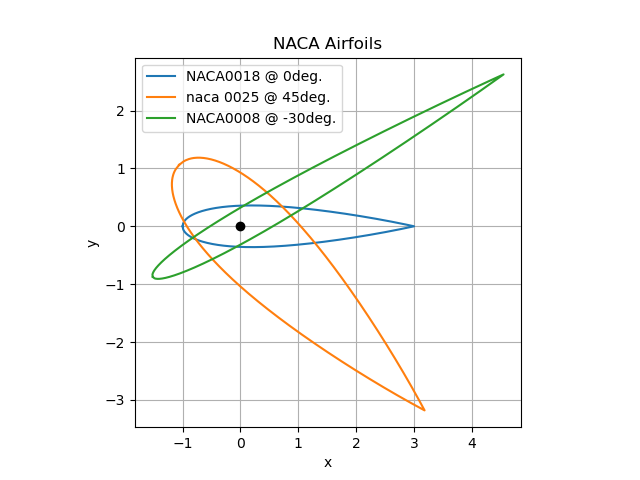
\includegraphics[width=0.75\textwidth]{exOutput.png}
\end{figure}

In addition, by running \texttt{computeAirfoils()}, the plot above is produced. Note that the quarter-chord positions of all airfoils are located at $(x,y) = (0,0)$, that a "positive" value of pitch corresponds to the leading edge pointing upward, and that the legend indicates the profile and pitch angle as provided to the function. Your plot should match the characteristics of that shown above: \textbf{it should have axis labels, a title, a grid, a legend, and have an "equal" aspect ratio} (e.g., one unit of $x$ has the same length as one unit of $y$, as in the real world). However, otherwise it does not need to be fancy (for example, you do not need to specify legend positioning, nor use a non-default color scheme), as the intent is mainly for you to practice basic plotting syntax.

\subsection*{Input Requirements}

Your \texttt{computeAirfoils()} function should be flexible in that it can accept the specifications of an arbitrary number of airfoils. These airfoil specifications should be provided as lists of values of the appropriate type. \textbf{However}, your code should also be able to handle the case of a single airfoil, where single values (rather than lists) may be provided. For example:

\begin{python}
foilCoords = computeAirfoils('NACA0018', 4, 6)
\end{python}

For any number of airfoils, the profile names provided may or may not be uppercase/lowercase (e.g., 'NACA0018' vs 'naca0018' vs 'nAcA0018'), and may or may not have a space in between 'NACA' and the specification digits (e.g., 'naca0018' vs 'naca 0018'). Consider how \texttt{str} methods can help you simply address these cases.

Additionally, your \texttt{computeAirfoils()} function should also be able to handle certain incorrect or incompatible inputs, and throw errors accordingly. To summarize, your function should be able to enforce the following conditions on its inputs:
\begin{enumerate}
    \item The number of profile names, number of chord lengths, and number of pitch angles provided to \texttt{computeAirfoils()} must all be equal. Otherwise, an \texttt{IndexError} should be thrown.
    
    \item The chord length(s) and pitch angle(s) must be specified as numeric values or as \texttt{lists} of numeric values. The airfoil profile name(s) (e.g., NACA 0018) must be specified as a \texttt{str} or a \texttt{list} of \texttt{str}. If values of other types are provided for these inputs, a \texttt{TypeError} should be thrown. You may assume that if an input has the correct type that its value is otherwise valid.
\end{enumerate}

You can raise a particular type of error via the following syntax:

\begin{python}
if (condition): # If we want to throw an error
    raise TypeError('Message that will be printed when error is thrown')
\end{python}

I recommend defining helper functions to handle these error cases, and calling them at the beginning of \texttt{computeAirfoils()} (see below). To check if a variable is of a particular type, use the \texttt{isinstance()} function. For example, to check if \texttt{x} is a list: \texttt{isinstance(x, list)}. Notice that we are providing the type name directly as \texttt{list}. To check if a value is numeric (rather than whether it is specifically an integer or a decimal), you can import the \texttt{numbers} module and use \texttt{numbers.Number} as the type name. Also, just as for the \texttt{isinstance()} function, you can pass type names directly to functions that you define. You should use this to develop a single, generalized type-checking function that you can use for each input.

\begin{python}
def computeAirfoils(profileNames, chords, angles)
    '''
    [docstring here]
    '''

    # Check inputs for correct typing
    anyOutputs = checkType(profileNames, additionalParameters...)
    anyOutputs = checkType(chords, additionalParameters...)
    anyOutputs = checkType(angles, additionalParameters...)

    # Check inputs for size compatibility
    checkSizes(profileNames, chords, angles)

    # The rest of your function
    ...
\end{python}

\subsubsection*{Style}

As always, your script will also be graded on whether it is well-structured and follows the Style Guide. All of the usual guidelines apply: you should factor out distinct and/or repetitive tasks into functions to improve organization and reduce redundancy, and \textbf{every} function must have a docstring that describes its parameters, returns, and other behavior. As we discussed in class, when working with multi-dimensional numpy arrays, it is important to describe what each dimension (e.g., the rows, columns, pages) represents in the docstrings of any functions that use them as parameters or returns.

As we have practiced in lecture, use pseudocode to outline the problem and break it down into smaller pieces. This will help you identify the "steps" of the problem, including sub-tasks that are well represented by helper functions. If you are unsure of where to start, you can also solve simple versions of the problem first, and then add complexity. For example, you could first write a script that computes the coordinates of a single airfoil, assuming inputs of the correct type and size. Then, you could generalize this to an arbitrary number of airfoils, still assuming correct inputs. Then, you could add error checking...and so on.

If you have any questions about general style requirements or the specific style requirements for this assignment, post them to the discussion board.

%%%%%%%%%%%%%%%%%%%%%%%%%%%%%%%%%%%%%%%%%%%%%%%%%%%%
\newpage
\question*{Creative Programming II}

[Question removed]

% Write a Python program related to your engineering pursuits that imports some data into Python, performs some processing/analysis, and produces a plot related to that processing/analysis. Your program can be related to your other classes (past or present), research, job/internship, extracurriculars, or any other engineering topic. If you have an idea for a program topic but are unsure if it is appropriate, post on the Homework 4 page of the discussion board. \textbf{Your code must be different from that which you submitted for Creative Programming on Homework 1 or for other previous assignments for this class, but it can expand on the same topic, if appropriate.}

% In addition to satisfying the requirements in the Style Guide, your program should meet the following requirements:

% \begin{itemize}
%     \item Import some kind of data into Python (NumPy provides several functions for this).
%     \item Process or analyze the data in some way.
%     \item Produce a plot using \texttt{matplotlib} or another plotting package.
%      \item Define and use $\sim4$ or more non-trivial functions (4 is not a strict requirement, as long as your code is well-structured, but this roughly corresponds to a function each for importing/formatting data, processing data, plotting data, and wrapping it all together).
% \end{itemize}

% Your program will be graded primarily based on how well someone who knows Python, but is not familiar with your code or topic, (i.e., your instructor) can read and understand your script, as well as interpret your plot. You should follow the Style Guide to accomplish this: use functions to organize your code, write complete docstrings for all functions, incorporate inline comments to describe smaller chunks of code as appropriate, and include a program summary. Utilize axis labels, legends, titles, etc. to communicate information in your plot, and to make sure that your plot can be understood by someone who cannot see your code.

% Additionally, your program should be able to run without requiring specialized hardware (e.g., connection to equipment that the instructor does not have access to). You are not restricted to the content we have covered; if you have Python experience and want to use content from later in the course or beyond, you may do so.

% Submit your program as a \texttt{.py} file or \texttt{.ipynb} file. Submit any supporting files (e.g., data files) as well if applicable.

\end{document}

